% Define metadata
\documentclass{template/thesis}
\Title{ĐỀ TÀI: CẢI THIỆN KHẢ NĂNG TỰ PHỤC HỒI CHO HỆ THỐNG KUBERNETES SỬ DỤNG HỌC TĂNG CƯỜNG}
\Title[en]{TOPIC: IMPROVING SELF-HEALING CAPABILITY FOR KUBERNETES SYSTEMS USING REINFORCEMENT LEARNING}

\ThesisType{BÁO CÁO ĐỒ ÁN MÔN HỌC}

\University{ĐẠI HỌC QUỐC GIA THÀNH PHỐ HỒ CHÍ MINH}
\CollegeOrDept{{TRƯỜNG ĐẠI HỌC CÔNG NGHỆ THÔNG TIN}}
\Faculty{KHOA MẠNG MÁY TÍNH VÀ TRUYỀN THÔNG}


\Author{NGUYỄN TIẾN PHÁT}{23521147}
\Author{LÊ TRUNG KIÊN}{23520797}
\Author{HUỲNH LÂM TUẤN PHONG}{23521162}

\Degree{Môn học:}
\Major{NT549 - Học máy tăng cường cho các hệ thống mạng}
% \MajorCode{123}
\ThesisYear{2026}
\ThesisLocation{TP. HỒ CHÍ MINH}

\Supervisor{TS. Huỳnh Văn Đặng}

\hypersetup{
	pdfencoding=auto,
	pdfauthor={Nhóm 14},
	pdfsubject={Môn học: NT549 - Học máy tăng cường cho các hệ thống mạng; Ngành: Mạng máy tính và truyền thông dữ liệu},
	pdftitle={Cải thiện khả năng tự phục hồi cho hệ thống Kubernetes sử dụng học tăng cường},
	pdfkeywords={}
}

\usepackage{listings}
\lstset{
  basicstyle=\ttfamily\footnotesize,
  breaklines=true,
  backgroundcolor=\color{gray!5},
  frame=single,
  keywordstyle=\color{blue},
  commentstyle=\color{gray!60!black},
  stringstyle=\color{orange!80!black},
  numbers=none,
  tabsize=2,
  showstringspaces=false
}

\begin{document}
\firstbeforepreface
\secondbeforepreface
\afterpreface

\chapter{Giới thiệu}
\label{c:intro}
\section{Giới thiệu đề tài.}

\subsection{Động cơ nghiên cứu}

Trong những năm gần đây, kiến trúc microservices và nền tảng container hóa đã trở thành xu hướng chủ đạo trong việc triển khai các hệ thống phân tán hiện đại. Kubernetes hiện là nền tảng orchestration phổ biến nhất, được sử dụng rộng rãi để quản lý container, tự động triển khai, mở rộng và vận hành hệ thống dịch vụ quy mô lớn. Một trong những đặc điểm quan trọng của Kubernetes là khả năng \textit{self-healing} (tự phục hồi), cho phép hệ thống tự động khởi động lại Pod lỗi, thay thế Pod bị crash hoặc điều phối workload sang Node khác khi xảy ra sự cố.

Tuy nhiên, cơ chế tự phục hồi mặc định của Kubernetes chủ yếu hoạt động dựa trên các rule cố định và các controller truyền thống. Trong các môi trường thực tế có tải động, số lượng dịch vụ lớn và lỗi xảy ra liên tục, các cơ chế này vẫn tồn tại nhiều hạn chế như:
\begin{itemize}
    \item Thời gian phục hồi chưa tối ưu.
    \item Không thích nghi tốt với nhiều loại lỗi đồng thời.
    \item Thiếu khả năng học hỏi từ dữ liệu lịch sử.
    \item Không tối ưu tài nguyên trong quá trình phục hồi.
\end{itemize}

Trong khi đó, Reinforcement Learning (RL) là một nhánh của Machine Learning cho phép tác nhân (agent) học cách ra quyết định tối ưu thông qua quá trình tương tác với môi trường. RL đã được ứng dụng trong nhiều bài toán tối ưu động như robot, mạng máy tính, quản lý tài nguyên cloud và tối ưu scheduling. Khả năng học chính sách tối ưu dựa trên trạng thái hệ thống giúp RL trở thành hướng tiếp cận tiềm năng cho bài toán self-healing trong Kubernetes.

Từ đó, đề tài “Ứng dụng Reinforcement Learning cho bài toán tự phục hồi hệ thống Kubernetes trong các kịch bản Pod failure và Node failure” được thực hiện nhằm nghiên cứu khả năng áp dụng RL để hỗ trợ ra quyết định phục hồi hệ thống hiệu quả hơn so với cơ chế mặc định.


\chapter{Tổng quan lý thuyết, nghiên cứu liên quan}
\label{c:cosolythuyet}
\section{Reinforcement Learning}

Reinforcement Learning (RL) là một nhánh của Machine Learning trong đó một tác nhân (agent) học cách ra quyết định thông qua quá trình tương tác với môi trường và nhận về phần thưởng từ môi trường. Mục tiêu của agent là tối đa hóa phần thưởng tích lũy.

Khác với supervised learning, RL không phụ thuộc vào dữ liệu gán nhãn mà học thông qua cơ chế thử và sai (trial-and-error). Sau mỗi hành động, agent sẽ nhận được reward từ môi trường để đánh giá chất lượng quyết định đã thực hiện.

\begin{figure}[h]
    \centering
    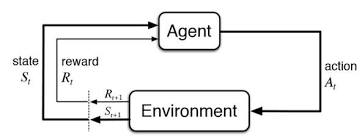
\includegraphics[width=0.7\textwidth]{img/RL.png}
    \caption{Mô hình cơ bản của Reinforcement Learning}
    \label{fig:ten_label}
\end{figure}


Một bài toán RL thường bao gồm các thành phần sau:
\begin{itemize}
    \item \textbf{State (S)}: Mô tả trạng thái hiện tại của môi trường.
    \item \textbf{Action (A)}: Tập các hành động mà agent có thể thực hiện.
    \item \textbf{Reward (R)}: Giá trị phản hồi từ môi trường sau khi agent thực hiện hành động.
    \item \textbf{Policy ($\pi$)}: Chiến lược lựa chọn hành động của agent.
    \item \textbf{Episode}: Chuỗi tương tác liên tục từ trạng thái khởi đầu đến trạng thái kết thúc.
\end{itemize}

Bài toán RL thường được mô hình hóa dưới dạng Markov Decision Process (MDP):

\[
MDP = (S, A, P, R, \gamma)
\]

Trong đó:

\begin{itemize}
    \item $S$: tập trạng thái.
    \item $A$: tập hành động.
    \item $P$: xác suất chuyển trạng thái.
    \item $R$: hàm reward.
    \item $\gamma$: hệ số discount factor.
\end{itemize}


\section{Thuật toán Deep Q-Network (DQN)}

Deep Q-Network (DQN) là thuật toán thuộc nhóm Deep Reinforcement Learning, được phát triển nhằm cải thiện Q-Learning trong các môi trường có không gian trạng thái lớn. Thay vì sử dụng bảng Q-Table, DQN sử dụng mạng neural sâu để xấp xỉ hàm giá trị hành động $Q(s,a)$.

Trong Reinforcement Learning, agent tương tác với môi trường thông qua trạng thái $s$, thực hiện hành động $a$, nhận phần thưởng $r$ và chuyển sang trạng thái tiếp theo $s'$. Mục tiêu của agent là tối đa hóa tổng phần thưởng tích lũy:

\[
R_t = \sum_{k=0}^{\infty} \gamma^k r_{t+k+1}
\]

Trong đó:
\begin{itemize}
    \item $R_t$: tổng phần thưởng tích lũy tại thời điểm $t$
    \item $\gamma$: hệ số discount factor $(0 < \gamma < 1)$
    \item $r_{t+k+1}$: phần thưởng trong tương lai
\end{itemize}

DQN sử dụng mạng neural để xấp xỉ hàm giá trị Q:

\[
Q(s,a;\theta)
\]

Trong đó:
\begin{itemize}
    \item $s$: trạng thái hiện tại
    \item $a$: hành động
    \item $\theta$: trọng số của mạng neural
\end{itemize}

Giá trị Q được cập nhật dựa trên phương trình Bellman:

\[
Q(s,a)=r+\gamma \max_{a'}Q(s',a')
\]

Trong đó:
\begin{itemize}
    \item $r$: phần thưởng nhận được
    \item $s'$: trạng thái tiếp theo
    \item $\gamma$: hệ số discount factor
    \item $\max_{a'}Q(s',a')$: giá trị Q lớn nhất tại trạng thái kế tiếp
\end{itemize}

Trong quá trình huấn luyện, DQN tối ưu giá trị dự đoán thông qua target value:

\[
y = r+\gamma \max_{a'}Q(s',a';\theta^{-})
\]

Trong đó:
\begin{itemize}
    \item $y$: giá trị mục tiêu
    \item $\theta^{-}$: trọng số của Target Network
\end{itemize}

Hàm mất mát (Loss Function) của DQN được xác định như sau:

\[
L(\theta)=\mathbb{E}\left[(y-Q(s,a;\theta))^2\right]
\]

Trong đó:
\begin{itemize}
    \item $Q(s,a;\theta)$: giá trị Q dự đoán từ mạng neural
    \item $y$: giá trị mục tiêu
\end{itemize}

Gradient được sử dụng để cập nhật trọng số mạng neural:

\[
\nabla_{\theta}L(\theta)=
\mathbb{E}\left[(y-Q(s,a;\theta))
\nabla_{\theta}Q(s,a;\theta)\right]
\]

Trong đó:
\begin{itemize}
    \item $y$: giá trị mục tiêu (target value)
    \item $Q(s,a;\theta)$: giá trị Q được dự đoán bởi mạng neural
    \item $\nabla_{\theta}Q(s,a;\theta)$: đạo hàm của hàm Q theo trọng số mạng neural
    \item $\theta$: tập trọng số của mạng neural
\end{itemize}

Để cân bằng giữa exploration và exploitation, DQN sử dụng chiến lược $\varepsilon$-greedy:

\[
a=
\begin{cases}
\text{random action}, & \text{with probability } \varepsilon \\
\arg\max_a Q(s,a), & \text{with probability } 1-\varepsilon
\end{cases}
\]



\section{Proximal Policy Optimization (PPO)}

Proximal Policy Optimization (PPO) là một thuật toán thuộc nhóm Policy Gradient trong Reinforcement Learning, được đề xuất bởi OpenAI nhằm cải thiện tính ổn định và hiệu quả trong quá trình huấn luyện policy. PPO được thiết kế để khắc phục các hạn chế của các phương pháp Policy Gradient truyền thống và Trust Region Policy Optimization (TRPO), đặc biệt là hiện tượng cập nhật policy quá lớn dẫn đến mất ổn định hoặc không hội tụ trong quá trình học.

PPO thuộc kiến trúc Actor--Critic, bao gồm hai thành phần chính là Actor và Critic. Actor chịu trách nhiệm học policy để lựa chọn hành động phù hợp với trạng thái hiện tại của môi trường, trong khi Critic có nhiệm vụ ước lượng giá trị của trạng thái thông qua hàm value function. Sự kết hợp giữa hai thành phần này giúp giảm phương sai (variance) của gradient và tăng độ ổn định trong quá trình huấn luyện.

\begin{figure}[!htbp]
\centering
\small
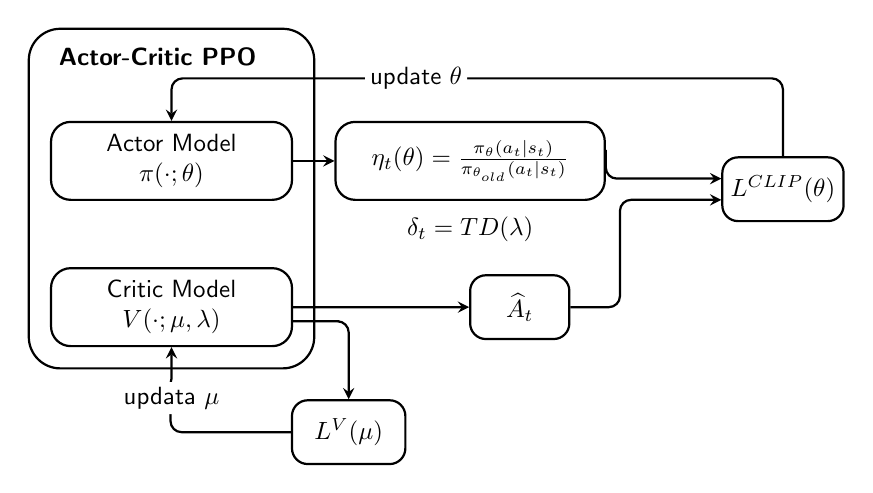
\begin{tikzpicture}[
    scale=0.9, transform shape,
    % Định nghĩa style các khối cố định độ rộng để text không làm phình node
    block/.style={
        draw=black, thick, rounded corners=2.5mm, 
        minimum width=3.4cm, minimum height=1.1cm, 
        align=center, fill=white, font=\sffamily
    },
    small/.style={
        draw=black, thick, rounded corners=2mm, 
        minimum width=1.4cm, minimum height=0.9cm, 
        align=center, fill=white, font=\sffamily
    },
    line/.style={
        ->, >=stealth, thick, rounded corners=4pt
    }
]

    % --- 1. NHÓM ACTOR & CRITIC (Gốc tọa độ) ---
    \node[block] (actor) at (0, 0) {Actor Model\\$\pi(\cdot ; \theta)$};
    % Đẩy Critic xuống dưới Actor cố định 1.5cm
    \node[block] (critic) at ([yshift=-1.5cm]actor.south) {Critic Model\\$V(\cdot ; \mu, \lambda)$};

    % Khung bao Actor-Critic PPO: Dựa hoàn toàn vào góc của actor và critic để không bao giờ bị lệch
    \draw[thick, rounded corners=4mm] 
        ([xshift=-0.3cm, yshift=1.3cm]actor.north west) rectangle ([xshift=0.3cm, yshift=-0.3cm]critic.south east);
    % Nhãn chữ đặt động ở giữa
    \node[font=\sffamily\bfseries, anchor=west] at ([yshift=0.9cm]actor.north west) {Actor-Critic PPO};
    
    % --- 2. CÁC KHỐI TÍNH TOÁN Ở GIỮA (Dịch chuyển theo trục X từ khối bên trái) ---
    % Khối eta_t nằm ngang hàng với Actor, cách sang phải 2.5cm
    \node[block, minimum width=3.8cm] (ratio) at ([xshift=2.5cm]actor.east) {$\eta_t(\theta) = \frac{\pi_\theta(a_t \mid s_t)}{\pi_{\theta_{\text{old}}}(a_t \mid s_t)}$};
    
    % Khối Advantage A_t nằm dịch sang phải từ Critic
    \node[small] (advantage) at ([xshift=3.2cm, yshift=0cm]critic.east) {$\widehat{A}_t$};
    
    % Nhãn delta_t nằm độc lập ngay dưới ratio
    \node (delta) at ([yshift=-0.4cm]ratio.south) [font=\sffamily] {$\delta_t = \text{TD}(\lambda)$};

    % --- 3. CÁC KHỐI LOSS (Nằm ngoài cùng và phía dưới) ---
    % Khối L^CLIP dịch sang phải từ khối ratio
    \node[small, minimum width=1.6cm] (l_clip) at ([xshift=2.5cm, yshift=-0.4cm]ratio.east) {$\text{L}^{\text{CLIP}}(\theta)$};
    
    % Khối L^V nằm ngay dưới khối Critic
    \node[small, minimum width=1.6cm] (l_v) at ([xshift=2.5cm, yshift=-1.2cm]critic.south) {$\text{L}^{\text{V}}(\mu)$};

    % --- 4. HỆ THỐNG ĐƯỜNG NỐI MŨI TÊN ---
    
    % Từ Actor thẳng sang Ratio
    \draw[line] (actor.east) -- (ratio.west);
    
    % Từ Critic sang Khối Advantage
    \draw[line] (critic.east) -- (advantage.west);
    
    % Từ Critic đi xuống thẳng khối L^V
    \draw[line] ([yshift=-0.2cm]critic.east) -- ++(0.5,0) -| (l_v.north);
    
    % Đường gom từ Ratio và Advantage vào L^CLIP
    \draw[line] (ratio.east) -- ++(0,0) |- ([yshift=0.15cm]l_clip.west);
    \draw[line] (advantage.east) -- ++(0.7,0) |- ([yshift=-0.15cm]l_clip.west);
    
    % --- 5. ĐƯỜNG PHẢN HỒI CẬP NHẬT (FEEDBACK LOOPS) ---

    % Update theta: Từ đỉnh L^CLIP vòng lên trên đỉnh Actor
    \draw[line] (l_clip.north) -- ++(0,1.1) -| (actor.north)
        node[pos=0.3, fill=white, inner sep=2pt, font=\sffamily] {update $\theta$};
         
    % Update mu: Từ đáy L^V đi vòng sang trái rồi đâm thẳng vào đáy Critic
    \draw[line] (l_v.west) -- ++(-1.7,0) |- ([yshift=-0.6cm]critic.south) -- (critic.south)
        node[pos=-0.2, fill=white, inner sep=2pt, font=\sffamily] {updata $\mu$};

\end{tikzpicture}
\caption{Sơ đồ hoàn chỉnh kiến trúc Actor-Critic PPO cấu trúc lại}
\label{fig:actor_critic_ppo_perfect}
\end{figure}


Trong Reinforcement Learning, policy là một phân phối xác suất ánh xạ từ trạng thái sang hành động:


\[
\pi(a|s)
\]

Trong đó:
\begin{itemize}
    \item $s$: trạng thái của môi trường
    \item $a$: hành động được lựa chọn
    \item $\pi(a|s)$: xác suất chọn hành động $a$ tại trạng thái $s$
\end{itemize}

Sau mỗi lần tương tác với môi trường, Critic ước lượng giá trị trạng thái nhằm hỗ trợ Actor cập nhật policy theo hướng tối ưu.

Hàm mục tiêu cơ bản của Policy Gradient được định nghĩa:

\[
J(\theta) = \mathbb{E}_{\pi_\theta}[R_t]
\]

Trong đó:
\begin{itemize}
    \item $J(\theta)$: hàm mục tiêu cần tối ưu
    \item $\pi_\theta$: policy với tham số $\theta$
    \item $R_t$: tổng reward tích lũy
\end{itemize}

Gradient của hàm mục tiêu:

\[
\nabla_\theta J(\theta)
= \mathbb{E}_{\pi_\theta}\left[\nabla_\theta \log \pi_\theta(a_t|s_t)\, R_t \right]
\]

Tuy nhiên, Policy Gradient truyền thống có phương sai cao và khó ổn định. Do đó, PPO sử dụng Advantage Function:

\[
A_t = Q(s_t, a_t) - V(s_t)
\]

Trong đó:
\begin{itemize}
    \item $Q(s_t, a_t)$: giá trị hành động
    \item $V(s_t)$: giá trị trạng thái
\end{itemize}

Nếu $A_t > 0$, hành động tốt hơn kỳ vọng.

Ngược lại nếu $A_t < 0$, hành động kém hơn kỳ vọng.

PPO định nghĩa probability ratio giữa policy mới và policy cũ:

\[
r_t(\theta) =
\frac{\pi_\theta(a_t|s_t)}{\pi_{\theta_{\text{old}}}(a_t|s_t)}
\]

Tỷ lệ này phản ánh mức độ thay đổi của policy giữa hai lần cập nhật.

Hàm objective chính của PPO (clipped surrogate objective):

\[
L^{CLIP}(\theta)
=
\mathbb{E}_t \left[
\min \Big(
r_t(\theta) A_t,\;
\text{clip}(r_t(\theta), 1-\epsilon, 1+\epsilon) A_t
\Big)
\right]
\]

Trong đó:
\begin{itemize}
    \item $r_t(\theta)$: probability ratio
    \item $A_t$: advantage estimate
    \item $\epsilon$: clipping parameter
\end{itemize}

Cơ chế clipping giới hạn mức thay đổi của policy trong khoảng $[1-\epsilon, 1+\epsilon]$, giúp tránh cập nhật quá lớn gây mất ổn định hoặc divergence.

Quá trình huấn luyện PPO gồm các bước:

Agent tương tác với môi trường, thu thập trajectory, tính reward và advantage, sau đó tối ưu hàm clipped objective bằng mini-batch gradient descent. Thuật toán thường thực hiện nhiều epoch trên cùng một batch dữ liệu nhằm tăng sample efficiency.

Nhờ cơ chế cập nhật ổn định và hiệu quả trong không gian trạng thái lớn, PPO là một trong những thuật toán Deep Reinforcement Learning được sử dụng phổ biến trong các bài toán điều khiển, quản lý tài nguyên và hệ thống phân tán.


\section{Các nghiên cứu liên quan}

Trong những năm gần đây, việc ứng dụng các mô hình học máy vào vấn đề tự phục hồi của các hệ thống phân tán vẫn đang là chủ đề mới

Trong bài “AI-enhanced self-healing Kubernetes for scalable cloud operations”, tác giả Veeresh Nunavath đã chỉ ra rằng mặc dù Kubernetes sở hữu các tính năng tự phục hồi tích hợp sẵn mạnh mẽ, chúng vẫn chỉ mang tính chất phản ứng và bị giới hạn về phạm vi. Nghiên cứu khẳng định việc tích hợp AI sẽ giúp cơ chế tự phục hồi truyền thống tiến hóa thành các hệ thống tự trị, có khả năng thích nghi và dự đoán lỗi. Tuy nhiên, bài viết chủ yếu dừng lại ở múc độ kiến trúc tổng thể và các chiến lược triển khai lý thuyết.

Nghiên cứu “Self-Healing Infrastructure: Leveraging Reinforcement Learning for Autonomous Cloud Recovery and Enhanced Resilience” đã đề xuất một khung cơ sở hạ tầng tự phục hồi đa tầng kết hợp giữa phân tích dự đoán và Reinforcement Learning (RL). Điểm đáng chú ý trong nghiên cứu này là dùng thuật toán PPO làm bộ não điều phối. Tác nhân PPO liên tục thu thập dữ liệu đo lường như CPU, RAM và network để đưa ra các hành động phục hồi động dựa trên một hàm phần thưởng đánh giá tính khả dụng của hệ thống.

Kế thừa các quan điểm từ hai nghiên cứu trên, đồ tài này sẽ tiếp tục đi sâu vào việc khai thác thuật toán PPO trong môi trường Kubernetes, tập trung thiết kế không gian trạng thái đa chiều và tinh chỉnh hàm phần thưởng nhằm giải quyết cho 5 kịch bản lỗi phổ biến trong kiến trúc microservices.




\chapter{Mô hình bài toán}
\label{c:mohinhbaitoan}
Phần này trình bày mô hình bài toán của đề tài, bao gồm mô tả hệ thống,
định nghĩa trạng thái, hành động, hàm thưởng và mục tiêu tối ưu.

% TODO: Cập nhật nội dung chi tiết Chương 3.


\chapter{Phương pháp đề xuất}
\label{c:phuongphapdexuat}
Chương này trình bày phương pháp đề xuất cho bài toán, bao gồm thuật toán sử dụng,
kiến trúc mô hình neural network, hàm mất mát, và quy trình huấn luyện.

% TODO:
% - Mô tả chi tiết thuật toán đề xuất
% - Trình bày kiến trúc mô hình
% - Định nghĩa hàm mất mát và mục tiêu tối ưu
% - Quy trình huấn luyện và tiêu chí dừng


\chapter{Cài đặt và thực nghiệm}
\label{c:caidatvathucnghiem}
\section{Thiết kế cơ sở hạ tầng trên nền tảng AWS}

Môi trường thực nghiệm được thiết kế và triển khai trên nền tảng Amazon Web Services (AWS) nhằm đảm bảo tính linh hoạt, khả năng mở rộng tự động và mức độ sẵn sàng cao (High Availability). Kiến trúc hệ thống phân bổ dịch vụ trên nhiều Vùng khả dụng (Availability Zones - AZs) trong cùng một VPC (Virtual Private Cloud) để triệt tiêu các điểm lỗi đơn lẻ (SPoF) và tối ưu hóa khả năng chịu lỗi vật lý.

Chi tiết mô hình kiến trúc hạ tầng AWS được minh họa cụ thể trong Hình \ref{fig:aws-infra-architecture}.

\begin{figure}[htbp]
    \centering
    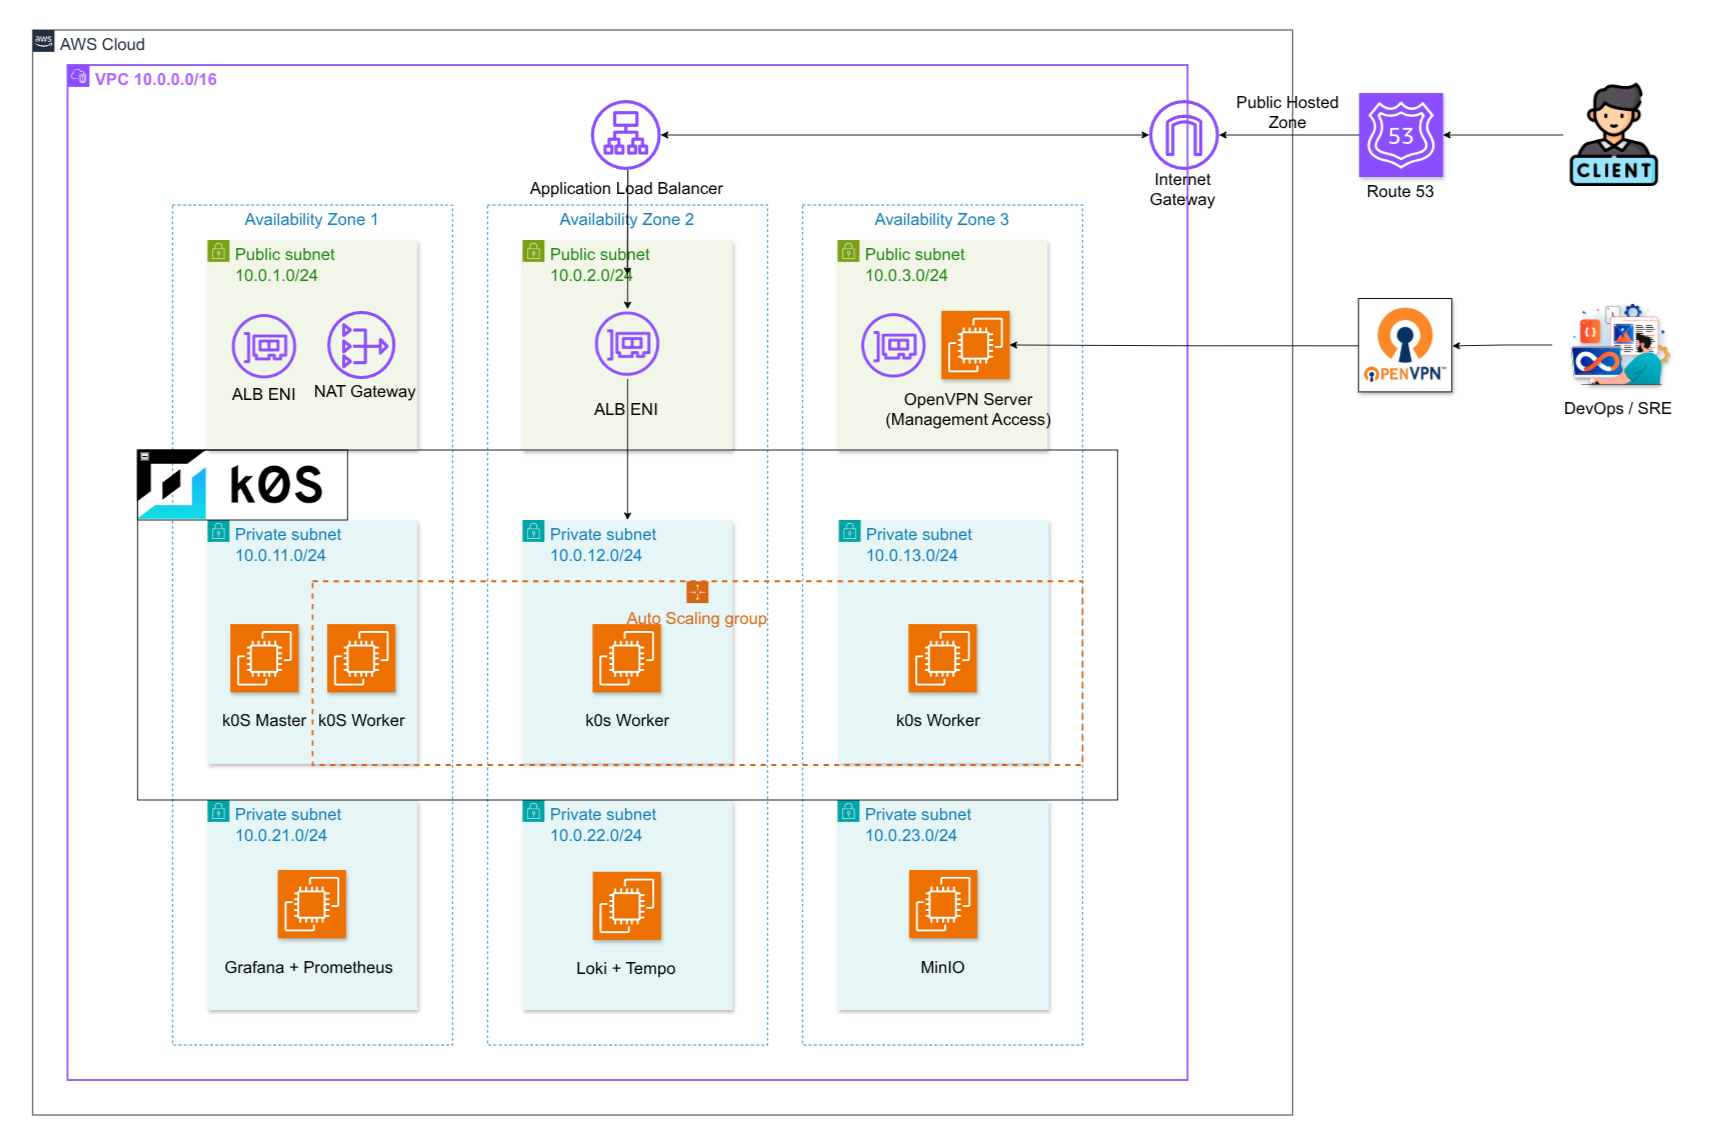
\includegraphics[width=0.8\textwidth]{graphics/chapter-5/cloud.png}
    \caption{Kiến trúc triển khai cơ sở hạ tầng trên nền tảng AWS}
    \label{fig:aws-infra-architecture}
\end{figure}

Kiến trúc hạ tầng bao gồm ba lớp chức năng chính:
\begin{itemize}
    \item \textbf{Lớp mạng (Networking Layer):} VPC dải mạng \texttt{10.0.0.0/16} được chia làm các Public/Private Subnet trên 03 AZs (us-east-1a, us-east-1b, us-east-1c). Lớp này sử dụng Internet Gateway (IGW) cho kết nối ngoài, NAT Gateway bảo mật cho phân vùng nội bộ, và Application Load Balancer (ALB) điều phối lưu lượng.
    \item \textbf{Lớp tính toán (Compute Layer):} Cụm Kubernetes được phân bổ trên cả 03 AZs để vận hành workloads. Trong đó, Master node đặt tại Private Subnet của AZ 1, các Worker node được phân tán ở các AZs khác nhau. Ngoài ra, hệ thống được bổ sung thêm Auto Scaling Group giúp hỗ trợ tăng giảm số máy Worker phục vụ lượng tải linh hoạt từ người dùng.
    \item \textbf{Lớp giám sát và quản trị (Management Layer):} Tích hợp Prometheus để thu thập dữ liệu huấn luyện (metrics) thời gian thực và Grafana để trực quan hóa phục vụ phân tích. Hệ thống quản trị được bảo mật thông qua OpenVPN Server đặt tại Public Subnet của AZ 3.
\end{itemize}

Để tối ưu hóa luồng lưu lượng và đảm bảo tính cô lập an toàn, chúng tôi thực hiện phân hoạch địa chỉ IP chi tiết cho toàn bộ các phân vùng mạng (Subnets) trong hệ thống như được trình bày trong Bảng \ref{tab:subnet-ip-allocation}.

\begin{center}
\captionof{table}{Phân hoạch địa chỉ IP cho các Subnets trong hệ thống thực nghiệm}
\label{tab:subnet-ip-allocation}
\footnotesize
\renewcommand{\arraystretch}{1.0}
\begin{tabular}{|C{3.2cm}|C{2.8cm}|C{3.0cm}|L{6.0cm}|}
\hline
\textbf{Vùng khả dụng (AZ)} & \textbf{Loại Subnet} & \textbf{Dải địa chỉ (CIDR)} & \textbf{Thành phần được triển khai} \\ \hline
\multirow{3}{*}{us-east-1a (AZ 1)} & Public & 10.0.1.0/24 & ALB ENI, NAT Gateway \\ \cline{2-4} 
 & Private (k0s) & 10.0.11.0/24 & k0s Master, k0s Worker Node \\ \cline{2-4} 
 & Private (Data) & 10.0.21.0/24 & Prometheus, Grafana \\ \hline
\multirow{3}{*}{us-east-1b (AZ 2)} & Public & 10.0.2.0/24 & ALB ENI \\ \cline{2-4} 
 & Private (k0s) & 10.0.12.0/24 & k0s Worker Node (Auto Scaling) \\ \cline{2-4} 
 & Private (Data) & 10.0.22.0/24 & Phân vùng dự phòng (Unused) \\ \hline
\multirow{3}{*}{us-east-1c (AZ 3)} & Public & 10.0.3.0/24 & OpenVPN Access Server \\ \cline{2-4} 
 & Private (k0s) & 10.0.13.0/24 & k0s Worker Node \\ \cline{2-4} 
 & Private (Data) & 10.0.23.0/24 & Phân vùng dự phòng (Unused) \\ \hline
\end{tabular}
\end{center}

Cơ sở hạ tầng mạng và tính toán này thiết lập một môi trường thực nghiệm có tính chân thực cao, tương đương với các hệ thống Cloud Production. Đây là nền tảng cốt lõi để thực hiện các kịch bản kích hoạt sự cố nhân tạo (Chaos Injection) liên quan đến \textit{Pod failure} và \textit{Node failure}, từ đó đo lường chính xác thời gian phục hồi và độ ổn định của giải pháp đề xuất so với cơ chế mặc định của Kubernetes.

\section{Triển khai cơ sở hạ tầng sử dụng Terraform}

Để đảm bảo tính tự động hóa, tính nhất quán và khả năng tái lập nhanh chóng cho môi trường thực nghiệm, toàn bộ tài nguyên hạ tầng trên AWS được định nghĩa và khởi tạo dưới dạng mã nguồn (Infrastructure as Code - IaC) thông qua công cụ Terraform. Việc này giúp triệt tiêu các sai sót cấu hình thủ công và kiểm soát chặt chẽ trạng thái tài nguyên thông qua tệp tin \texttt{terraform.tfstate}.


Quy trình áp dụng hạ tầng được thực hiện qua các lệnh tiêu chuẩn của Terraform bao gồm: \texttt{terraform init} (khởi tạo môi trường), \texttt{terraform plan} (kiểm tra dự báo thay đổi) và \texttt{terraform apply} (thực thi khởi tạo thực tế trên AWS). 


\section{Cấu hình các công cụ sử dụng Ansible}

Để tự động hóa cấu hình hệ điều hành và thiết lập phần mềm trên các máy chủ EC2 đã được khởi tạo bởi Terraform, chúng tôi sử dụng công cụ Ansible. Với kiến trúc không tác nhân (\textit{agentless}), Ansible thực hiện truyền tải các cấu hình thông qua kết nối SSH bảo mật, giúp thiết lập môi trường đồng bộ, nhất quán và giảm thiểu tối đa các thao tác quản trị thủ công. Các chỉ thị cấu hình được khai báo dưới dạng tệp tin YAML (\textit{Ansible Playbooks}).

\subsection{Cấu hình dịch vụ mạng riêng ảo sử dụng OpenVPN}

Dịch vụ OpenVPN Server được cấu hình và thiết lập tự động thông qua Ansible trên máy chủ đặt tại Public Subnet của AZ 3. Vai trò của thành phần này là thiết lập một đường truyền mã hóa bảo mật từ xa (VPN Tunnel) cho phép quản trị viên truy cập an toàn vào dải mạng nội bộ (Private Subnet) của VPC để thực hiện các thao tác quản trị cụm Kubernetes và hệ thống giám sát mà không cần công khai các cổng dịch vụ ra Internet.

\subsection{Cấu hình cụm Kubernetes}

Quy trình thiết lập cụm Kubernetes được tự động hóa hoàn toàn bằng Ansible Playbook bao gồm các công đoạn chính:
\begin{itemize}
    \item \textbf{Chuẩn bị môi trường:} Tắt phân vùng swap, cấu hình các tham số nhân hệ điều hành (\textit{sysctl}) cho mạng container và cài đặt container runtime (như \texttt{containerd}).
    \item \textbf{Cấu hình Master Node:} Khởi tạo nút điều khiển (Control Plane), thiết lập tệp cấu hình \texttt{kubeconfig} và cài đặt Container Network Interface (CNI) để thiết lập mạng nội bộ cho các Pods.
    \item \textbf{Gia nhập các Worker Nodes:} Ansible tự động trích xuất mã thông báo gia nhập (\textit{join token}) từ Master Node và thực thi lệnh kết nối các Worker Nodes phân tán trên các AZs vào cụm.
\end{itemize}

\subsection{Cấu hình hệ thống giám sát sử dụng Prometheus và Grafana}

Hệ thống giám sát được cấu hình tập trung trên máy chủ chuyên dụng đặt tại Private Subnet của AZ 1 nhằm đảm bảo tính toàn vẹn dữ liệu:
\begin{itemize}
    \item \textbf{Prometheus:} Được cấu hình thông qua Ansible để tự động phát hiện dịch vụ (\textit{service discovery}) trong cụm Kubernetes, thu thập dữ liệu metrics từ \texttt{node-exporter} (được Ansible cài đặt trên từng node) và \texttt{kube-state-metrics} theo chu kỳ 15 giây.
    \item \textbf{Grafana:} Được cấu hình sẵn các nguồn dữ liệu (\textit{Data Sources}) kết nối trực tiếp tới Prometheus và tự động nạp các bảng giao diện trực quan hóa (\textit{Dashboards}) để theo dõi hiệu năng tài nguyên hệ thống (CPU, RAM, Network) theo thời gian thực.
\end{itemize}


\chapter{Kết quả và phân tích}
\label{c:ketquavaphantich}
Chương này trình bày kết quả thực nghiệm và phân tích, bao gồm biểu đồ quá trình
huấn luyện, so sánh giữa các thuật toán, và đánh giá kết quả đạt được.

% TODO:
% - Biểu đồ training (reward/loss theo episode)
% - So sánh với baseline
% - Phân tích điểm mạnh, điểm yếu


\chapter{Kết luận và hướng phát triển}
\label{c:ketluanvahuongphattrien}
\input{chapters/7-KetLuanVaHuongPhatTrien}

\begingroup
\setlength{\emergencystretch}{8em}
\justifying\printbibliography[title=Tài liệu tham khảo]
\endgroup
\addcontentsline{toc}{chapter}{Tài liệu tham khảo}



\end{document}
